%%%%%%%%%%%%%%%%%%%%%%%%%%%%%%%%%% Preâmbulo %%%%%%%%%%%%%%%%%%%%%%%%%%%%%%%%%% 

\documentclass[12pt,a4paper]{article}\usepackage[]{graphicx}\usepackage[]{color}
% maxwidth is the original width if it is less than linewidth
% otherwise use linewidth (to make sure the graphics do not exceed the margin)
\makeatletter
\def\maxwidth{ %
  \ifdim\Gin@nat@width>\linewidth
    \linewidth
  \else
    \Gin@nat@width
  \fi
}
\makeatother

\definecolor{fgcolor}{rgb}{0.345, 0.345, 0.345}
\newcommand{\hlnum}[1]{\textcolor[rgb]{0.686,0.059,0.569}{#1}}%
\newcommand{\hlstr}[1]{\textcolor[rgb]{0.192,0.494,0.8}{#1}}%
\newcommand{\hlcom}[1]{\textcolor[rgb]{0.678,0.584,0.686}{\textit{#1}}}%
\newcommand{\hlopt}[1]{\textcolor[rgb]{0,0,0}{#1}}%
\newcommand{\hlstd}[1]{\textcolor[rgb]{0.345,0.345,0.345}{#1}}%
\newcommand{\hlkwa}[1]{\textcolor[rgb]{0.161,0.373,0.58}{\textbf{#1}}}%
\newcommand{\hlkwb}[1]{\textcolor[rgb]{0.69,0.353,0.396}{#1}}%
\newcommand{\hlkwc}[1]{\textcolor[rgb]{0.333,0.667,0.333}{#1}}%
\newcommand{\hlkwd}[1]{\textcolor[rgb]{0.737,0.353,0.396}{\textbf{#1}}}%
\let\hlipl\hlkwb

\usepackage{framed}
\makeatletter
\newenvironment{kframe}{%
 \def\at@end@of@kframe{}%
 \ifinner\ifhmode%
  \def\at@end@of@kframe{\end{minipage}}%
  \begin{minipage}{\columnwidth}%
 \fi\fi%
 \def\FrameCommand##1{\hskip\@totalleftmargin \hskip-\fboxsep
 \colorbox{shadecolor}{##1}\hskip-\fboxsep
     % There is no \\@totalrightmargin, so:
     \hskip-\linewidth \hskip-\@totalleftmargin \hskip\columnwidth}%
 \MakeFramed {\advance\hsize-\width
   \@totalleftmargin\z@ \linewidth\hsize
   \@setminipage}}%
 {\par\unskip\endMakeFramed%
 \at@end@of@kframe}
\makeatother

\definecolor{shadecolor}{rgb}{.97, .97, .97}
\definecolor{messagecolor}{rgb}{0, 0, 0}
\definecolor{warningcolor}{rgb}{1, 0, 1}
\definecolor{errorcolor}{rgb}{1, 0, 0}
\newenvironment{knitrout}{}{} % an empty environment to be redefined in TeX

\usepackage{alltt}
\usepackage[utf8]{inputenc}
\usepackage{amsmath}
\usepackage{amsfonts}
\usepackage{amssymb}
\usepackage{makeidx}
\usepackage{graphicx}
\usepackage{booktabs}
\usepackage{xcolor}
\usepackage{bm}
\usepackage{float}
\usepackage[margin=1.5in]{geometry}
\let\lctau\tau % save the lowercase of '\tau'
\renewcommand{\tau}{\scalerel*{\lctau}{X}}

\usepackage{hyperref}
\hypersetup{
    colorlinks,
    citecolor=black,
    filecolor=black,
    linkcolor=black,
    urlcolor=black
}

\renewcommand{\contentsname}{Sumário} 

\title{MLG - Trabalho 2}
\author{José Carlos Soares Junior }
\date{Matrícula: 2017100732}
\IfFileExists{upquote.sty}{\usepackage{upquote}}{}
\begin{document}
\begin{titlepage}
	\begin{center}
	
	%\begin{figure}[!ht]
	%\centering
	%\includegraphics[width=2cm]{c:/ufba.jpg}
	%\end{figure}

		\Huge{UNIVERSIDADE FEDERAL DO ESPÍRITO SANTO}\\
		\large{CENTRO DE CIÊNCIAS EXATAS}\\ 
		\large{DEPARTAMENTO DE ESTATÍSTICA}\\ 
\vspace{15pt}
        
        \vspace{85pt}
        
		\textbf{\LARGE{Modelagem dos dados de 2013 referentes às notificações de dengue no estado do Espírito Santo}}
		\title{\large{Título}}
	%	\large{Modelo\\
     %   		Validação do modelo clássico}
			
	\end{center}
\vspace{1,5cm}
	
	\begin{flushright}

   \begin{list}{}{
      \setlength{\leftmargin}{4.5cm}
      \setlength{\rightmargin}{0cm}
      \setlength{\labelwidth}{0pt}
      \setlength{\labelsep}{\leftmargin}}

      \item Segundo trabalho da disciplina de MLG ministrado pelo Prof. Dr. Saulo Morellato.

      \begin{list}{}{
      \setlength{\leftmargin}{0cm}
      \setlength{\rightmargin}{0cm}
      \setlength{\labelwidth}{0pt}
      \setlength{\labelsep}{\leftmargin}}

			\item Alunos: \
            \item Orientador: Prof. Dr. Saulo Morellato\

      \end{list}
   \end{list}
\end{flushright}
\vspace{1cm}
\begin{center}
		\vspace{\fill}
		 Abril\\
		 2021
			\end{center}
\end{titlepage}
\newpage

%%%%%%%%%%%%%%%%%%%%%%%%%%%%%%%%%% Pacotes %%%%%%%%%%%%%%%%%%%%%%%%%%%%%%%%%% 



\tableofcontents  % sumário

% Formato do chunk a ser usado:



%%%%%%%%%%%%%%%%%%%%%%%%%%% Descrição dos dados %%%%%%%%%%%%%%%%%%%%%%%%%%%%%% 

\newpage
\section{\textbf{{\LARGE\textbf{Descrição dos dados}}}}

\textbf{IntCdAtBca} - Proporção de internações por condições sensíveis à Atenção Basica;

\noindent
\textbf{CobCondSaud} - Cobertura de acompanhamento das condicionalidades de saúde do Programa Bolsa Família;

\noindent
\textbf{CobAtBas} - Cobertura das equipes atenção básica municipal expresso em percentual da cobertura populacional alcançada pela Atenção Básica;

\noindent
\textbf{temp} - temperatura média anual;

\noindent
$\mathbf{temp\_p10}$ - percentil $10$ das temperaturas durante o ano;

\noindent
$\mathbf{temp\_p90}$ - percentil $90$ das temperaturas durante o ano;

\noindent
\textbf{precip} - precipitação pluviométrica acumulada anual;

\noindent
\textbf{umid} - média anual da umidade relativa do ar;

\noindent
$\mathbf{umid\_p10}$ - percentil $10$ da umidade relativa do ar durante o ano;

\noindent
$\mathbf{umid\_p90}$ - percentil $90$ da umidade relativa do ar durante o ano;

\noindent
\textbf{alt} - altitude da sede municipal;

\noindent
\textbf{ifdm\_saude} - Índice Firjan de Desenvolvimento Municipal-IFDM para saúde;

\noindent
\textbf{ifdm\_edu} - Índice Firjan de Desenvolvimento Municipal-IFDM para educação;

\noindent
\textbf{ifdm\_emprend} - Índice Firjan de Desenvolvimento Municipal-IFDM de emprego e renda;

\noindent
\textbf{cobveg} - índice de cobertura vegetal;

\noindent
\textbf{expcosteira} - ídice de exposição costeira;

\noindent
\textbf{ivc} - índice de vulnerabilidade climática;

\noindent
\textbf{pobr} - proporção de pobres;

\noindent
\textbf{ExpAnosEstud} - expectativa de anos de estudo;

\noindent
\textbf{urb} - proporção da população que reside em zona urbana;

\noindent
$\mathbf{menor15}$ - proporção da população com menos de $15$ anos;

\noindent
$\mathbf{maior65}$ - proporção da população com mais de $65$ anos;

\noindent
\textbf{adultos} - proporção da população entre $15$ e $65$ anos;

\noindent
\textbf{pop} - população do município;

\noindent
\textbf{area} - área do município;

\noindent
\textbf{dens} - densidade populacional (pop\/area);

\noindent
\textbf{id} - identificação;

\noindent
\textbf{ano} - ano referente às informações; e

\noindent
\textbf{dengue} - número de notificações municipais de dengue.

%%%%%%%%%%%%%%%%%%%%%%%%%%%%%%%%%% Descritiva %%%%%%%%%%%%%%%%%%%%%%%%%%%%%%%%%% 

\newpage
\section{{\LARGE\textbf{Análise exploratória}}}

%%%%%% Notificações de dengue por municipio %%%%%%%

\begin{knitrout}
\definecolor{shadecolor}{rgb}{0.969, 0.969, 0.969}\color{fgcolor}

{\centering 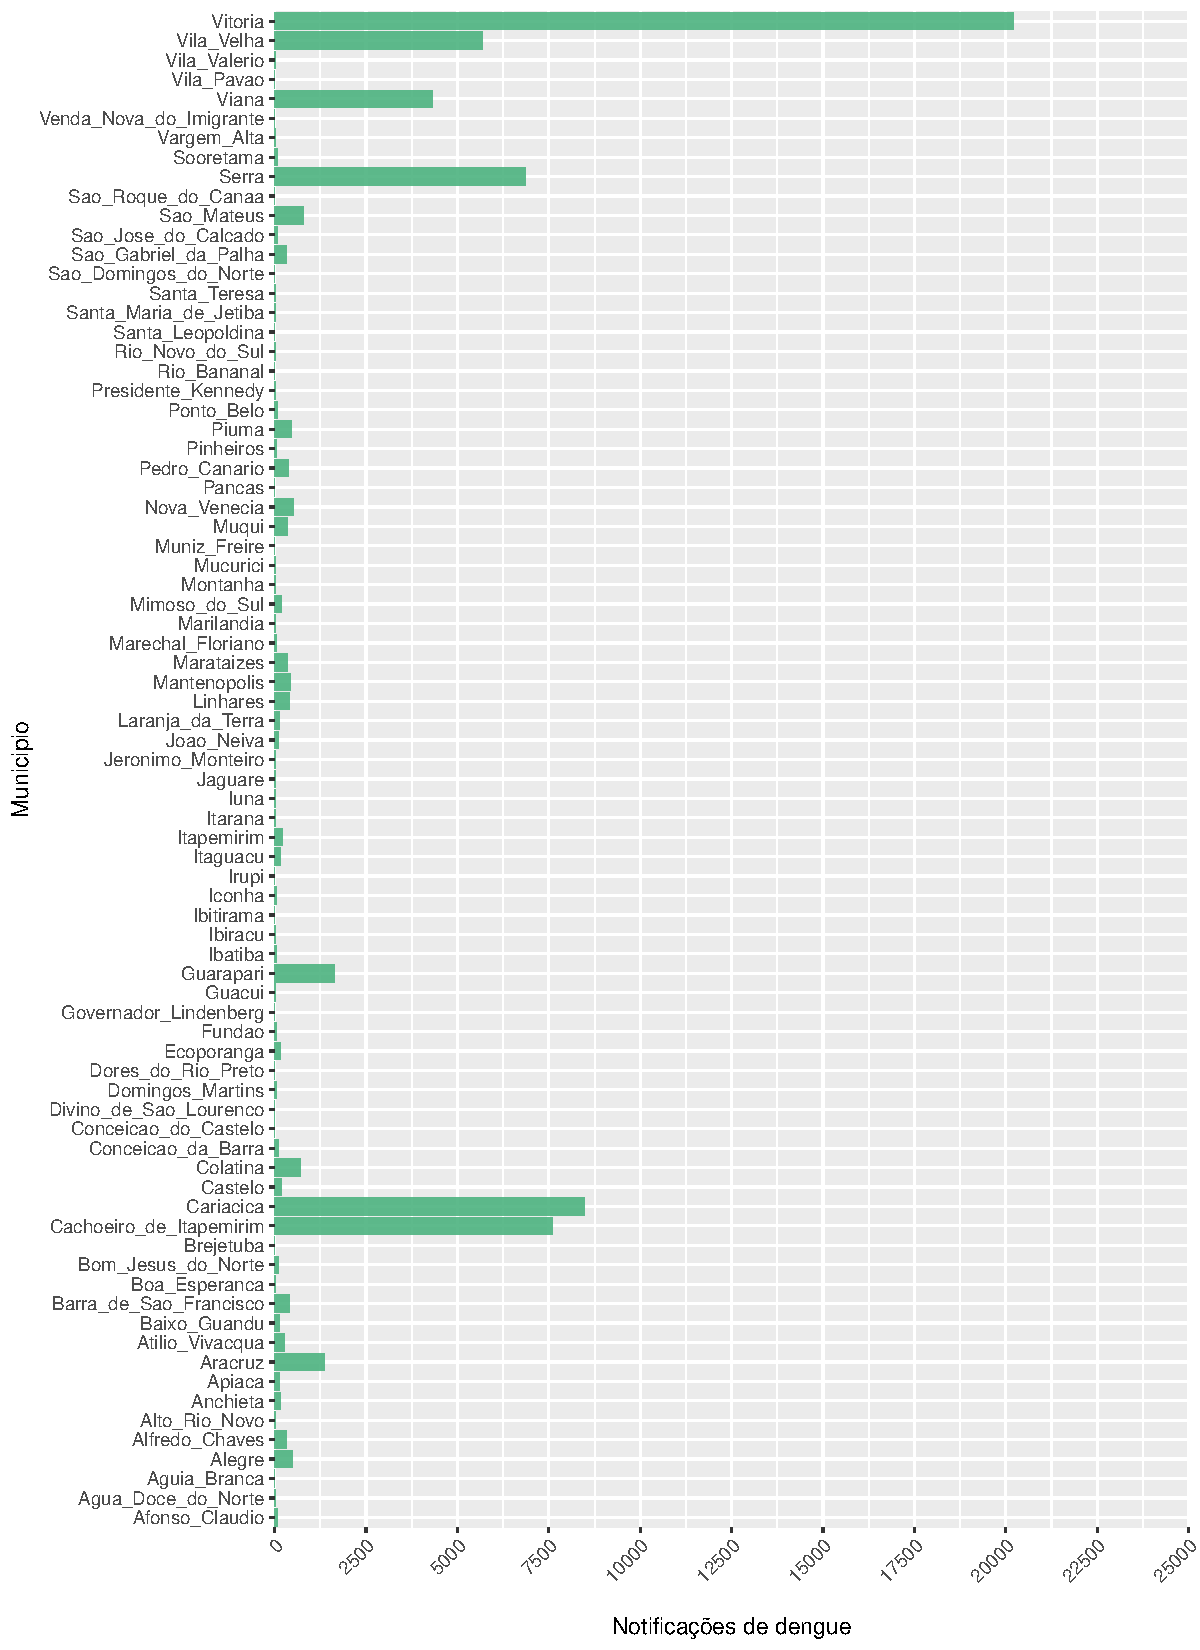
\includegraphics[width=\maxwidth]{figure/unnamed-chunk-3-1} 

}



\end{knitrout}
\textbf{Figura 1:} Notificações de dengue por municípios do estado do Espírito Santo.

%%%%%%% Grafico de correlação %%%%%%%

\begin{knitrout}
\definecolor{shadecolor}{rgb}{0.969, 0.969, 0.969}\color{fgcolor}
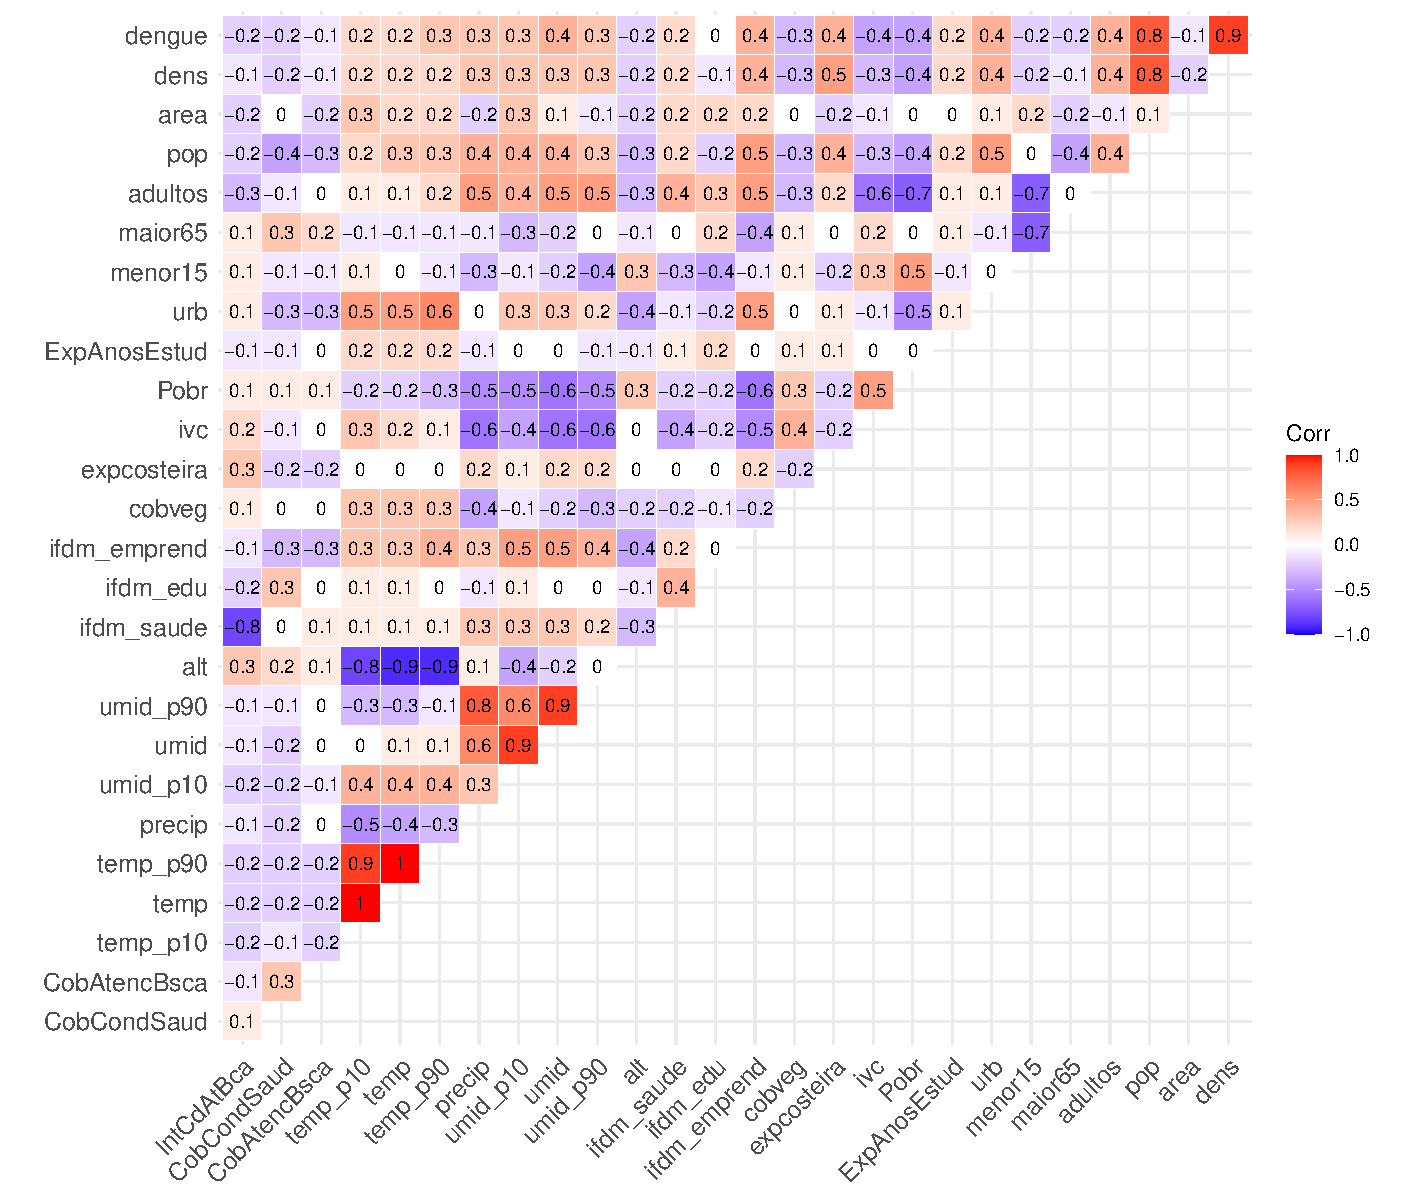
\includegraphics[width=\maxwidth]{figure/unnamed-chunk-4-1} 

\end{knitrout}
\textbf{Figura 2:} Gráfico de correlação entre as covariáveis.

\newpage
\section{{\LARGE\textbf{Construção do modelo}}}

\subsection{\textbf{Definição do modelo}}

\subsection{\textbf{Modelo considerando todas as covariáveis}}

\subsection{\textbf{Verificando multicolinearidade}}




\subsection{\textbf{Seleção de covariáveis}}


\subsection{\textbf{Transformação de covariáveis}}

\newpage
\subsection{\textbf{Pontos influentes/de alavanca/outliers}}

\newpage
\section{{\LARGE\textbf{Verificação dos pressupostos}}}

\newpage
\section{{\LARGE\textbf{Interpretação e conclusões}}}

\end{document}
